In the fallowing chapter the workflow described in chapter~\ref{ch:workflow} is carried out based on the current project status of \textit{Odoo}\footnote{https://www.odoo.com/}. \textit{Odoo} (formerly known as OpenERP) is a suite of \textit{open-source}\footnote{https://github.com/odoo/odoo} enterprise applications, targeting companies of all sizes. As each costumer needs different functionalities from \textit{Odoo}, the product variations can be very different in size and target use. Besides them researching in the field of easing their product configuration process, this project suits our workflows requirements.

The current version of \textit{Odoo} (version 9.0, released \mbox{October 1, 2015)} has 465~contributors and over 101.200~commits. They have developed 266 features which are all inside of a top hierarchy folder named ``addons''. Each of them contain code as well as a configuration file named ``\_\_openerp\_\_.py''. Inside this file there are all the relevant informations for this feature, like dependencies, summaries , categories, versions and more descriptive informations. Inside the \textit{Odoo} repository there are also other directories, like ``doc'' for documentary files, ``setup'' for deployment scripts on various platforms and ``openerp'' with the core code. However, as the variability is only contained within the features, the only relevant directory for this work is ``addons''.

At first, a feature model is generated based on the naming conventions of the project folders and the configuration files contained therein. Afterwards the feature model is corrected from any errors that occurred during the generation process. The resulting model combined with domain knowledge allows for the creation of a questionnaire that takes a minimum of choices to configure a custom tailored application.

All the \textit{Odoo} features lie inside of a folder named "addons". The code of each feature is contained in its own folder which is named like the parent feature with a suffix of its own name. According to this naming convention the feature "website\textunderscore sale" is a child of the feature "website", and parent to "website\textunderscore sale\textunderscore stock". In addition to the naming convention, there is a configuration file, written in python in each of the feature folders. These files contain a description of the feature, a name, that doesn't always match with the folder name and the dependencies that are required for this feature to work.
By first creating a list of all features based on the folder names, we can match them to the names inside of the configuration files. At this point we realize, that there are some conflicts in the naming of the 261 features. For example the feature "sale" is a standalone feature and has nothing to do with the sale from the feature "event\textunderscore sale". As the default FeatureIDE doesn't support multiple features with the same name, we decided to leave the full names with the underscores. In addition, there are some folder names where the underscore doesn't separate features, like "point\textunderscore of\textunderscore sale". For those we implemented naming exceptions where the user can add strings that represent a single feature.

We applied these steps to a total of 261 folders, containing in total more than 18.800 files, extracting 306 features. The surplus features result from abstract features, that do not have their own folder, but are implicit in the naming. The resulting feature model is arranged in a total of six hierarchical levels. Additionally, 196 constraints limit the possible valid configurations of \textit{Odoo}.

The choices made by the user have to be evaluated. This happens after each single question got answered. Especially the validity needs to be ensured at every time. Optimally, the questionnaire gets designed in such a way, that it is impossible to create an invalid configuration by just answering it. However, as the questionnaire itself does not get checked for validity, checking the answers adds that needed reassurance for validity. To check for validity, the dependencies assigned to a selected answer are checked. If a dependency-feature is previously unselected (undefined), it get (de-) selected according to the definition in the questionnaire. But if is already is in a state of (de-) selection, that doesn't match the state assigned in the questionnaire, an error occurs and warns the user of an invalid configuration.

As stated in Section~\ref{ch:quest-impl}, it is possible to define a dynamic ordering of the questions within the questionnaire according to the given answer. The next step in evaluating the user input is looking for the correct question to be asked next. If there is a next question explicitly stated in the selected answer, that question gets displayed next. Else, if there are questions left unanswered in the questionnaire, that occur after the current questions, the question displayed next is the question following the current question in the definition. If there is no next question to be displayed, the questionnaire is considered finished. Optimally, this also results in a final configuration of a product. However, our design also allows for partial configurations as a result of an executed questionnaire. In the case of a finished configuration, this configuration gets passed to FeatureIDE, which then compiles the configured product.


\begin{figure}
	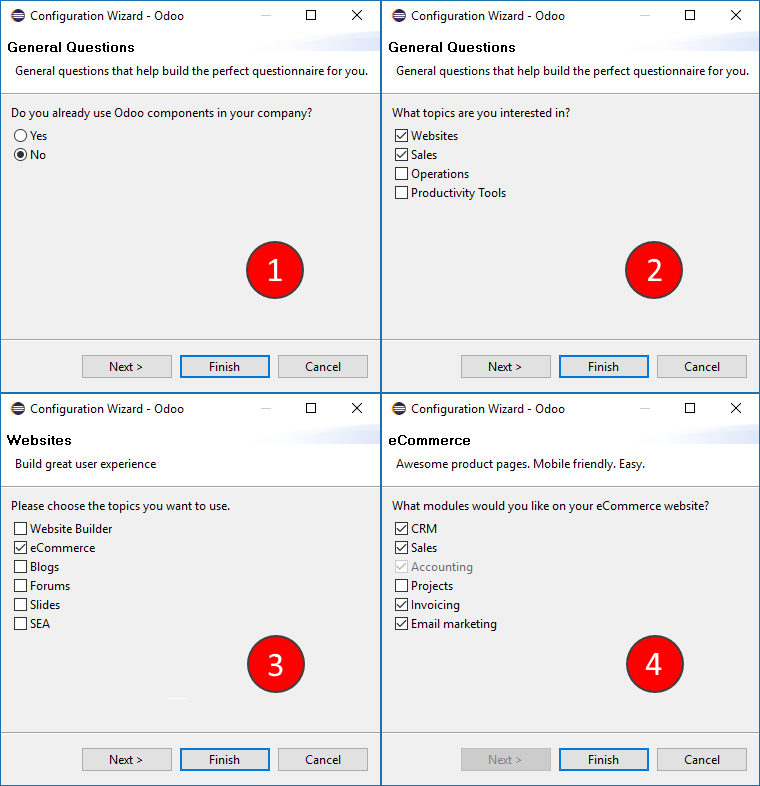
\includegraphics[width=\columnwidth]{img/img-screenshots.png}
	\caption{Screen shots of the questionnaire dialog while configuring Odoo}
	\label{img-screenshots}
\end{figure}

{\color{red}TODO: Fragebogen}


%TODO: Auswertung

%Also state how some of the questions and their mapping in the questionnaire were developed.

%Finally, show the process of configuration through running a fictinal user over the questionnaire and document his decisions as well as the resulting configurations.

%TODO: test ausdenken, der alle ``Fähgkeiten'' zeigt

% Fahrradladen, Online-Shop, Social-Media, Bezahldienste, Kontakt-Portal, DE/EN, Newsletter
%
% Website builder, eCommerce, SEA
% Sales, CRM, invoicing, Point of Sale
% Inventory, Purchase
% Email Marketing, Survey

%TODO: Planung, durchführung, Auswertung

%TODO: nur ein konstruierter Fall, weil Domain Knowledge fehlt.